\documentclass{whiteboard}
\begin{document}
\begin{frame}[plain,t]
 \bbcover{OJ 1112}{Mice and Maze}{Prof. Edson Alves}{Faculdade UnB Gama}
\end{frame}

\begin{frame}[plain,t]
\vspace*{\fill}
 \bbenglish{A set of laboratory mice is being trained to escape a maze. The maze is made up of cells, and each cell is connected to some other cells. However, there are obstacles in the passage between cells and therefore there is a time penalty to overcome the passage. Also, some passages allow mice to go one-way, but not the other way round.}

 \vspace{0.1in}

 \bbenglish{Suppose that all mice are now trained and, when placed in an arbitrary cell in the maze, take a path that leads them to the exit cell in minimum time.}
\vspace*{\fill}
\end{frame}

\begin{frame}[plain,t]
\vspace*{\fill}
 \bbtext{Um conjunto de ratos de laboratório está sendo treinado para escapar de um labirinto. O labirinto é formado por celas, e cada cela está conectada a algumas outras celas. Contudo, há obstáculos nas passagens entre as celas e portanto há uma penalidade de tempo para atravessar a passagem. Além disso, algumas passagens permitem aos ratos seguir em uma direção, mas não na direção contrária.}

 \vspace{0.1in}

 \bbtext{Suponha que todos os ratos estejam treinados e, quando postos em uma cela arbitrária do labirinto, eles escolhem o caminho que os leva a saída no menor tempo possível.}
\vspace*{\fill}
\end{frame}

\begin{frame}[plain,t]
\vspace*{\fill}
 \bbenglish{We are going to conduct the following experiment: a mouse is placed in each cell of the maze and a count-down timer is started. When the timer stops we count the number of mice out of the maze.}

 \vspace{0.1in}

 \bbenglish{Write a program that, given a description of the maze and the time limit, predicts the number of mice that will exit the maze. Assume that there are no bottlenecks in the maze, i.e. that all cells have room for an arbitrary number of mice.}
\vspace*{\fill}
\end{frame}

\begin{frame}[plain,t]
\vspace*{\fill}
 \bbtext{Vamos conduzir o seguinte experimento: um rato será colocado em cada uma das celas do labirinto e um temporizador será iniciado. Quando o temporizador finalizar sua contagem decrescente contaremos o número de ratos que conseguiu escapar do labirinto. }

 \vspace{0.1in}

 \bbtext{Escreva um programa que, dada a descrição do labirinto e o limite de tempo, compute o número de ratos que irão escapar do labirinto. Assuma que não há gargalos no labirinto, isto é, que todas as celas tem espaço suficiente para um número arbitrário de ratos.}
\vspace*{\fill}
\end{frame}

\begin{frame}[plain,t]
\vspace*{\fill}
 \bbbold{Input}

 \vspace{0.1in}

 \bbenglish{The input begins with a single positive integer on a line by itself indicating the number of the cases following, each of them as described below. This line is followed by a blank line, and there is also a blank line between two consecutive inputs.}

 \vspace{0.1in}

 \bbenglish{The maze cells are numbered $1, 2, \ldots, N$, where $N$ is the total number of cells. You can assume that $N\leq 100$.}

 \vspace{0.1in}

 \bbenglish{The first three input lines contain $N$, the number of cells in the maze, $E$, the number of the exit cell, and the starting value $T$ for the count-down timer (in some arbitrary time unit).}
\vspace*{\fill}
\end{frame}

\begin{frame}[plain,t]
\vspace*{\fill}
 \bbbold{Entrada}

 \vspace{0.1in}

 \bbtext{A entrada começa com uma linha contendo um único inteiro positivo, o qual indica o número de casos de teste que se seguem, cada um deles descritos como indicado abaixo. Esta linha é seguida por uma linha em branco, e há uma linha em branco entre dois casos de teste consecutivos.}

 \vspace{0.1in}

 \bbtext{As celas do labirinto são numeradas $1, 2, \ldots, N$, onde $N$ é o número total de celas. Você pode assumir que $N\leq 100$.}

 \vspace{0.1in}

 \bbtext{As três primeiras linhas de um caso de teste contém o inteiro $N$, o número de celas no labirinto, $E$, o número da cela onde está a saída, e o valor inicial $T$ do temporizador (em alguma unidade de tempo arbitrária).}
\vspace*{\fill}
\end{frame}

\begin{frame}[plain,t]
\vspace*{\fill}
 \bbbold{Input}

 \vspace{0.1in}

 \bbenglish{The fourth line contains the number $M$ of connections in the maze, and is followed by $M$ lines, each specifying a connection with three integer numbers: two cell numbers $a$ and $b$ (in the range $1, \ldots, N$) and the number of time units it takes to travel from $a$ to $b$.}

 \vspace{0.1in}

 \bbenglish{Notice that each connection is one-way, i.e., the mice can’t travel from $b$ to $a$ unless there is another line specifying that passage. Notice also that the time required to travel in each direction might be different.}
\vspace*{\fill}
\end{frame}

\begin{frame}[plain,t]
\vspace*{\fill}
 \bbbold{Entrada}

 \vspace{0.1in}

 \bbtext{A quarta linha contém o número $M$ de passagens no labirinto, e é seguida por $M$ linhas, cada uma especificando uma passagem por meio de três números inteiros: os números das celas $a$ e $b$ (no intervalo $1, \ldots, N$) e o tempo necessário para ir da cela $a$ para a cela $b$.}

 \vspace{0.1in}

 \bbtext{Note que cada passagem é de mão única, isto é, os ratos não podem ir de $b$ para $a$ a menos que exista uma outra linha especificando esta passagem. Note também que o tempo necessário para atravessar a passagem em uma direção pode ser diferente do tempo necessário para atravessá-la na outra direção.}
\vspace*{\fill}
\end{frame}

\begin{frame}[plain,t]
\vspace*{\fill}
 \bbbold{Output}

 \vspace{0.1in}

 \bbenglish{For each test case, the output must follow the description below. The outputs of two consecutive cases will be separated by a blank line.}

 \vspace{0.1in}

 \bbenglish{The output consists of a single line with the number of mice that reached the exit cell $E$ in at most $T$ time units.}
\vspace*{\fill}
\end{frame}

\begin{frame}[plain,t]
\vspace*{\fill}
 \bbbold{Saída}

 \vspace{0.1in}

 \bbtext{Para cada caso de teste, a saída deve seguir a descrição abaixo. As saídas de dois casos de teste consecutivos devem ser separadas por uma linha em branco.}

 \vspace{0.1in}

 \bbtext{A saída consiste em uma única linha com o número de ratos que chegaram a saída $E$ em, no máximo, $T$ unidades de tempo.}
\vspace*{\fill}
\end{frame}

\begin{frame}[plain,t]
\begin{tikzpicture}
\node[draw,opacity=0] at (0, 0) {x};
\node[draw,opacity=0] at (14, 8) {x};
 \node[anchor=west] at (0, 7.5) { \bbbold{Exemplo de entrada e saída} };
\end{tikzpicture}
\end{frame}

\begin{frame}[plain,t]
\begin{tikzpicture}
\node[draw,opacity=0] at (0, 0) {x};
\node[draw,opacity=0] at (14, 8) {x};
 \node[anchor=west] at (0, 7.5) { \bbbold{Exemplo de entrada e saída} };
 \node[anchor=west] at (1, 6.5) { \bbtext{1} };
\end{tikzpicture}
\end{frame}

\begin{frame}[plain,t]
\begin{tikzpicture}
\node[draw,opacity=0] at (0, 0) {x};
\node[draw,opacity=0] at (14, 8) {x};
 \node[anchor=west] at (0, 7.5) { \bbbold{Exemplo de entrada e saída} };
 \node[anchor=west] at (1, 6.5) { \bbtext{1} };
 \node[anchor=west] at (2.25, 6.5) { \footnotesize \bbcomment{\# de casos de teste} };
 \draw[->,color=BBViolet] (1.5, 6.5) -- (2.25, 6.5);
\end{tikzpicture}
\end{frame}

\begin{frame}[plain,t]
\begin{tikzpicture}
\node[draw,opacity=0] at (0, 0) {x};
\node[draw,opacity=0] at (14, 8) {x};
 \node[anchor=west] at (0, 7.5) { \bbbold{Exemplo de entrada e saída} };
 \node[anchor=west] at (1, 6.5) { \bbtext{1} };
 \node[anchor=west] at (1, 5.5) { \bbtext{4} };
\end{tikzpicture}
\end{frame}

\begin{frame}[plain,t]
\begin{tikzpicture}
\node[draw,opacity=0] at (0, 0) {x};
\node[draw,opacity=0] at (14, 8) {x};
 \node[anchor=west] at (0, 7.5) { \bbbold{Exemplo de entrada e saída} };
 \node[anchor=west] at (1, 6.5) { \bbtext{1} };
 \node[anchor=west] at (1, 5.5) { \bbtext{4} };
 \node[anchor=west] at (2.25, 5.5) { \footnotesize \bbcomment{\# de celas} };
 \draw[->,color=BBViolet] (1.5, 5.5) -- (2.25, 5.5);
\end{tikzpicture}
\end{frame}

\begin{frame}[plain,t]
\begin{tikzpicture}
\node[draw,opacity=0] at (0, 0) {x};
\node[draw,opacity=0] at (14, 8) {x};
 \node[anchor=west] at (0, 7.5) { \bbbold{Exemplo de entrada e saída} };
 \node[anchor=west] at (1, 6.5) { \bbtext{1} };
 \node[anchor=west] at (1, 5.5) { \bbtext{4} };
 \node[anchor=west] at (2.25, 5.5) { \footnotesize \bbcomment{\# de celas} };
 \draw[->,color=BBViolet] (1.5, 5.5) -- (2.25, 5.5);
 \node[draw,very thick,circle] (A) at (6, 4) { \bbtext{1} };
 \node[draw,very thick,circle] (B) at (9, 7) { \bbtext{2} };
 \node[draw,very thick,circle] (C) at (12, 4) { \bbtext{3} };
 \node[draw,very thick,circle] (D) at (9, 1) { \bbtext{4} };
\end{tikzpicture}
\end{frame}

\begin{frame}[plain,t]
\begin{tikzpicture}
\node[draw,opacity=0] at (0, 0) {x};
\node[draw,opacity=0] at (14, 8) {x};
 \node[anchor=west] at (0, 7.5) { \bbbold{Exemplo de entrada e saída} };
 \node[anchor=west] at (1, 6.5) { \bbtext{1} };
 \node[anchor=west] at (1, 5.5) { \bbtext{4} };
 \node[draw,very thick,circle] (A) at (6, 4) { \bbtext{1} };
 \node[draw,very thick,circle] (B) at (9, 7) { \bbtext{2} };
 \node[draw,very thick,circle] (C) at (12, 4) { \bbtext{3} };
 \node[draw,very thick,circle] (D) at (9, 1) { \bbtext{4} };
 \node[anchor=west] at (1, 5.0) { \bbtext{2} };
\end{tikzpicture}
\end{frame}

\begin{frame}[plain,t]
\begin{tikzpicture}
\node[draw,opacity=0] at (0, 0) {x};
\node[draw,opacity=0] at (14, 8) {x};
 \node[anchor=west] at (0, 7.5) { \bbbold{Exemplo de entrada e saída} };
 \node[anchor=west] at (1, 6.5) { \bbtext{1} };
 \node[anchor=west] at (1, 5.5) { \bbtext{4} };
 \node[draw,very thick,circle] (A) at (6, 4) { \bbtext{1} };
 \node[draw,very thick,circle] (B) at (9, 7) { \bbtext{2} };
 \node[draw,very thick,circle] (C) at (12, 4) { \bbtext{3} };
 \node[draw,very thick,circle] (D) at (9, 1) { \bbtext{4} };
 \node[anchor=west] at (1, 5.0) { \bbtext{2} };
 \node[anchor=west] at (2.25, 5.0) { \footnotesize \bbcomment{\# da saída} };
 \draw[->,color=BBViolet] (1.5, 5.0) -- (2.25, 5.0);
\end{tikzpicture}
\end{frame}

\begin{frame}[plain,t]
\begin{tikzpicture}
\node[draw,opacity=0] at (0, 0) {x};
\node[draw,opacity=0] at (14, 8) {x};
 \node[anchor=west] at (0, 7.5) { \bbbold{Exemplo de entrada e saída} };
 \node[anchor=west] at (1, 6.5) { \bbtext{1} };
 \node[anchor=west] at (1, 5.5) { \bbtext{4} };
 \node[anchor=west] at (1, 5.0) { \bbtext{2} };
 \node[anchor=west] at (2.25, 5.0) { \footnotesize \bbcomment{\# da saída} };
 \draw[->,color=BBViolet] (1.5, 5.0) -- (2.25, 5.0);
 \node[draw,very thick,circle] (A) at (6, 4) { \includegraphics[scale=0.03]{figs/mouse.png} };
 \node[draw,very thick,circle] (B) at (9, 7) { \faFlagCheckered };
 \node[draw,very thick,circle] (C) at (12, 4) { \includegraphics[scale=0.03]{figs/mouse.png} };
 \node[draw,very thick,circle,fill=BBCyan] (D) at (9, 1) { \includegraphics[scale=0.03]{figs/mouse.png} };
\end{tikzpicture}
\end{frame}

\begin{frame}[plain,t]
\begin{tikzpicture}
\node[draw,opacity=0] at (0, 0) {x};
\node[draw,opacity=0] at (14, 8) {x};
 \node[anchor=west] at (0, 7.5) { \bbbold{Exemplo de entrada e saída} };
 \node[anchor=west] at (1, 6.5) { \bbtext{1} };
 \node[anchor=west] at (1, 5.5) { \bbtext{4} };
 \node[anchor=west] at (1, 5.0) { \bbtext{2} };
 \node[anchor=west] at (2.25, 5.0) { \footnotesize \bbcomment{\# da saída} };
 \draw[->,color=BBViolet] (1.5, 5.0) -- (2.25, 5.0);
 \node[draw,very thick,circle] (A) at (6, 4) { \includegraphics[scale=0.03]{figs/mouse.png} };
 \node[draw,very thick,circle] (B) at (9, 7) { \faFlagCheckered };
 \node[draw,very thick,circle] (C) at (12, 4) { \includegraphics[scale=0.03]{figs/mouse.png} };
 \node[draw,very thick,circle,fill=BBCyan] (D) at (9, 1) { \includegraphics[scale=0.03]{figs/mouse.png} };
\end{tikzpicture}
\end{frame}

\begin{frame}[plain,t]
\begin{tikzpicture}
\node[draw,opacity=0] at (0, 0) {x};
\node[draw,opacity=0] at (14, 8) {x};
 \node[anchor=west] at (0, 7) { \Large \bbbold{Solução} };
\end{tikzpicture}
\end{frame}

\begin{frame}[plain,t]
\begin{tikzpicture}
\node[draw,opacity=0] at (0, 0) {x};
\node[draw,opacity=0] at (14, 8) {x};
 \node[anchor=west] at (0, 7) { \Large \bbbold{Solução} };
 \node[anchor=west] at (1, 6) { \bbtext{Como computar o caminho máximo usando Bellman-Ford?} };
\end{tikzpicture}
\end{frame}

\begin{frame}[plain,t]
\begin{tikzpicture}
\node[draw,opacity=0] at (0, 0) {x};
\node[draw,opacity=0] at (14, 8) {x};
 \node[anchor=west] at (0, 7) { \Large \bbbold{Solução} };
 \node[anchor=west] at (1, 6) { \bbtext{Como computar o caminho máximo usando Bellman-Ford?} };
 \node[anchor=west] at (1.5, 5) { \bbcomment{Inverta o sinal das arestas e compute o caminho mínimo!} };
\end{tikzpicture}
\end{frame}

\begin{frame}[plain,t]
\begin{tikzpicture}
\node[draw,opacity=0] at (0, 0) {x};
\node[draw,opacity=0] at (14, 8) {x};
 \node[anchor=west] at (0, 7) { \Large \bbbold{Solução} };
 \node[anchor=west] at (1, 6) { \bbtext{Como computar o caminho máximo usando Bellman-Ford?} };
 \node[anchor=west] at (1.5, 5) { \bbcomment{Inverta o sinal das arestas e compute o caminho mínimo!} };
 \node[draw,very thick,circle] (A) at (1, 3) { \bbtext{A} };
 \node[draw,very thick,circle] (B) at (3, 1) { \bbtext{B} };
 \node[draw,very thick,circle] (C) at (5, 3) { \bbtext{C} };
 \draw[-latex,very thick,dashed,color=BBCyan] (A) to node[above] { \textcolor{BBOrange}{4} } (C);
 \draw[-latex,thick] (A) to node[below left] { \textcolor{BBOrange}{2} } (B);
 \draw[-latex,thick] (B) to node[below right] { \textcolor{BBOrange}{3} } (C);
\end{tikzpicture}
\end{frame}

\begin{frame}[plain,t]
\begin{tikzpicture}
\node[draw,opacity=0] at (0, 0) {x};
\node[draw,opacity=0] at (14, 8) {x};
 \node[anchor=west] at (0, 7) { \Large \bbbold{Solução} };
 \node[anchor=west] at (1, 6) { \bbtext{Como computar o caminho máximo usando Bellman-Ford?} };
 \node[anchor=west] at (1.5, 5) { \bbcomment{Inverta o sinal das arestas e compute o caminho mínimo!} };
 \node[draw,very thick,circle] (A) at (1, 3) { \bbtext{A} };
 \node[draw,very thick,circle] (B) at (3, 1) { \bbtext{B} };
 \node[draw,very thick,circle] (C) at (5, 3) { \bbtext{C} };
 \draw[-latex,very thick,dashed,color=BBCyan] (A) to node[above] { \textcolor{BBOrange}{4} } (C);
 \draw[-latex,thick] (A) to node[below left] { \textcolor{BBOrange}{2} } (B);
 \draw[-latex,thick] (B) to node[below right] { \textcolor{BBOrange}{3} } (C);
 \draw[-latex,very thick] (6, 2) to (8, 2);
\end{tikzpicture}
\end{frame}

\begin{frame}[plain,t]
\begin{tikzpicture}
\node[draw,opacity=0] at (0, 0) {x};
\node[draw,opacity=0] at (14, 8) {x};
 \node[anchor=west] at (0, 7) { \Large \bbbold{Solução} };
 \node[anchor=west] at (1, 6) { \bbtext{Como computar o caminho máximo usando Bellman-Ford?} };
 \node[anchor=west] at (1.5, 5) { \bbcomment{Inverta o sinal das arestas e compute o caminho mínimo!} };
 \node[draw,very thick,circle] (A) at (1, 3) { \bbtext{A} };
 \node[draw,very thick,circle] (B) at (3, 1) { \bbtext{B} };
 \node[draw,very thick,circle] (C) at (5, 3) { \bbtext{C} };
 \draw[-latex,very thick,dashed,color=BBCyan] (A) to node[above] { \textcolor{BBOrange}{4} } (C);
 \draw[-latex,thick] (A) to node[below left] { \textcolor{BBOrange}{2} } (B);
 \draw[-latex,thick] (B) to node[below right] { \textcolor{BBOrange}{3} } (C);
 \draw[-latex,very thick] (6, 2) to (8, 2);
 \node[draw,very thick,circle] (A) at (9, 3) { \bbtext{A} };
 \node[draw,very thick,circle] (B) at (11, 1) { \bbtext{B} };
 \node[draw,very thick,circle] (C) at (13, 3) { \bbtext{C} };
 \draw[-latex,thick] (A) to node[above] { \bbinfo{-4} } (C);
 \draw[-latex,very thick,dashed,color=BBCyan] (A) to node[below left] { \bbinfo{-2} } (B);
 \draw[-latex,very thick,dashed,color=BBCyan] (B) to node[below right] { \bbinfo{-3} } (C);
\end{tikzpicture}
\end{frame}

\begin{frame}[plain,t]
\begin{tikzpicture}
\node[draw,opacity=0] at (0, 0) {x};
\node[draw,opacity=0] at (14, 8) {x};
 \node[anchor=west] at (0, 7) { \Large \bbbold{Solução} };
\end{tikzpicture}
\end{frame}

\begin{frame}[plain,t]
\begin{tikzpicture}
\node[draw,opacity=0] at (0, 0) {x};
\node[draw,opacity=0] at (14, 8) {x};
 \node[anchor=west] at (0, 7) { \Large \bbbold{Solução} };
 \node[anchor=west] at (1, 6) { \bbtext{Como identificar ao menos um elemento de um ciclo negativo? } };
\end{tikzpicture}
\end{frame}

\begin{frame}[plain,t]
\begin{tikzpicture}
\node[draw,opacity=0] at (0, 0) {x};
\node[draw,opacity=0] at (14, 8) {x};
 \node[anchor=west] at (0, 7) { \Large \bbbold{Solução} };
 \node[anchor=west] at (1, 6) { \bbtext{Como identificar ao menos um elemento de um ciclo negativo? } };
 \node[anchor=west] at (1.5, 5) { \bbcomment{Se $\dist[u]$ é atualizado no Round \#$|V|$, então $u$ pertence a } };
 \node[anchor=west] at (3.5, 4.5) { \bbcomment{ao menos um ciclo negativo! } };
\end{tikzpicture}
\end{frame}

\begin{frame}[plain,t]
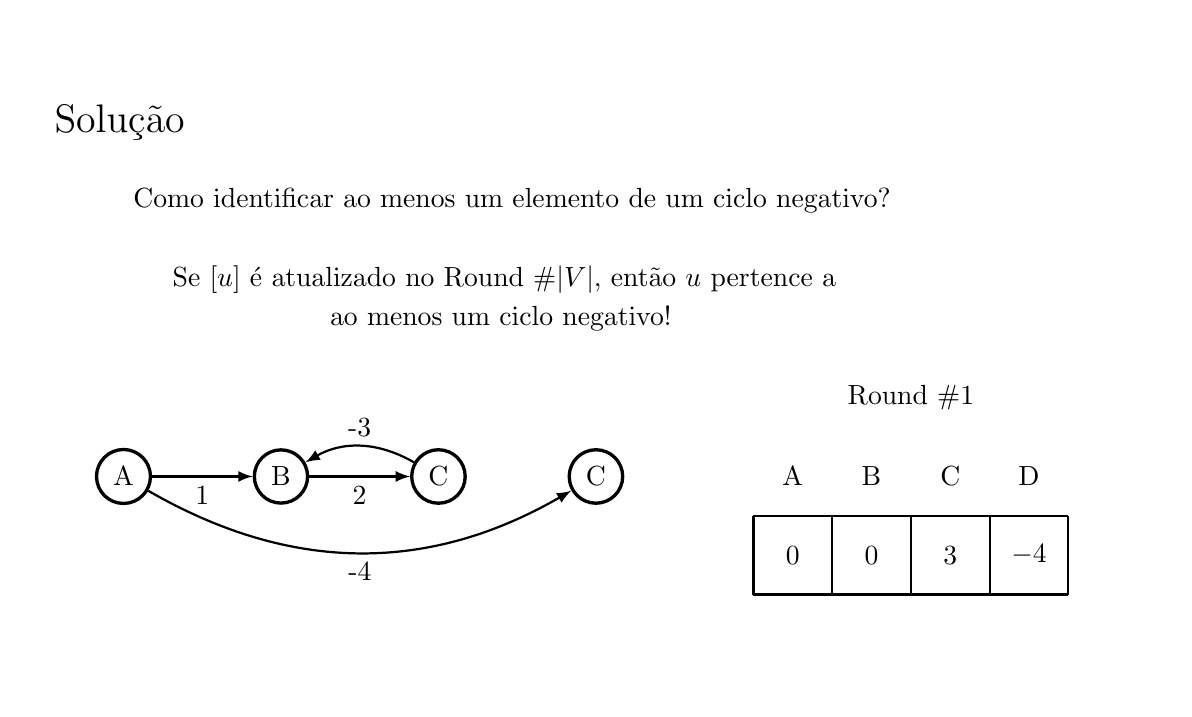
\begin{tikzpicture}
\node[draw,opacity=0] at (0, 0) {x};
\node[draw,opacity=0] at (14, 8) {x};
 \node[anchor=west] at (0, 7) { \Large \bbbold{Solução} };
 \node[anchor=west] at (1, 6) { \bbtext{Como identificar ao menos um elemento de um ciclo negativo? } };
 \node[anchor=west] at (1.5, 5) { \bbcomment{Se $\dist[u]$ é atualizado no Round \#$|V|$, então $u$ pertence a } };
 \node[anchor=west] at (3.5, 4.5) { \bbcomment{ao menos um ciclo negativo! } };
 \node[draw,very thick,circle] (A) at (1, 2.5) { \bbtext{A} };
 \node[draw,very thick,circle] (B) at (3, 2.5) { \bbtext{B} };
 \node[draw,very thick,circle] (C) at (5, 2.5) { \bbtext{C} };
 \node[draw,very thick,circle] (D) at (7, 2.5) { \bbtext{C} };
 \draw[-latex,thick] (A) to node[below] { \bbinfo{1} } (B);
 \draw[-latex,thick] (B) to node[below] { \bbinfo{2} } (C);
 \draw[-latex,thick] (C) to [bend right] node[above] { \bbinfo{-3} } (B);
 \draw[-latex,thick] (A) to [bend right] node[below] { \bbinfo{-4} } (D);
 \draw[thick] (9, 1) grid (13, 2);
 \node at (9.5, 2.5) { \bbtext{A} };
 \node at (10.5, 2.5) { \bbtext{B} };
 \node at (11.5, 2.5) { \bbtext{C} };
 \node at (12.5, 2.5) { \bbtext{D} };
 \node at (11, 3.5) { \bbbold{Round \#1} };
 \node at (9.5, 1.5) { $0$ };
 \node at (10.5, 1.5) { $0$ };
 \node at (11.5, 1.5) { $3$ };
 \node at (12.5, 1.5) { $-4$ };
\end{tikzpicture}
\end{frame}

\begin{frame}[plain,t]
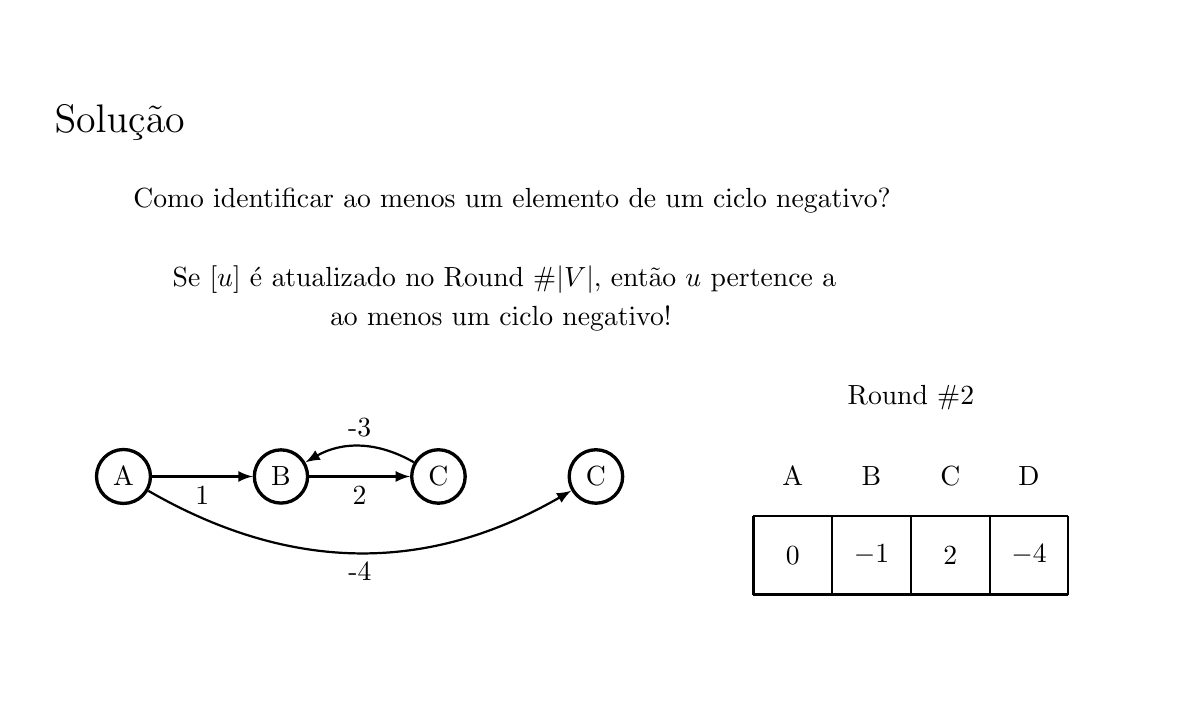
\begin{tikzpicture}
\node[draw,opacity=0] at (0, 0) {x};
\node[draw,opacity=0] at (14, 8) {x};
 \node[anchor=west] at (0, 7) { \Large \bbbold{Solução} };
 \node[anchor=west] at (1, 6) { \bbtext{Como identificar ao menos um elemento de um ciclo negativo? } };
 \node[anchor=west] at (1.5, 5) { \bbcomment{Se $\dist[u]$ é atualizado no Round \#$|V|$, então $u$ pertence a } };
 \node[anchor=west] at (3.5, 4.5) { \bbcomment{ao menos um ciclo negativo! } };
 \node[draw,very thick,circle] (A) at (1, 2.5) { \bbtext{A} };
 \node[draw,very thick,circle] (B) at (3, 2.5) { \bbtext{B} };
 \node[draw,very thick,circle] (C) at (5, 2.5) { \bbtext{C} };
 \node[draw,very thick,circle] (D) at (7, 2.5) { \bbtext{C} };
 \draw[-latex,thick] (A) to node[below] { \bbinfo{1} } (B);
 \draw[-latex,thick] (B) to node[below] { \bbinfo{2} } (C);
 \draw[-latex,thick] (C) to [bend right] node[above] { \bbinfo{-3} } (B);
 \draw[-latex,thick] (A) to [bend right] node[below] { \bbinfo{-4} } (D);
 \draw[thick] (9, 1) grid (13, 2);
 \node at (9.5, 2.5) { \bbtext{A} };
 \node at (10.5, 2.5) { \bbtext{B} };
 \node at (11.5, 2.5) { \bbtext{C} };
 \node at (12.5, 2.5) { \bbtext{D} };
 \node at (9.5, 1.5) { $0$ };
 \node at (12.5, 1.5) { $-4$ };
 \node at (11, 3.5) { \bbbold{Round \#2} };
 \node at (10.5, 1.5) { $-1$ };
 \node at (11.5, 1.5) { $2$ };
\end{tikzpicture}
\end{frame}

\begin{frame}[plain,t]
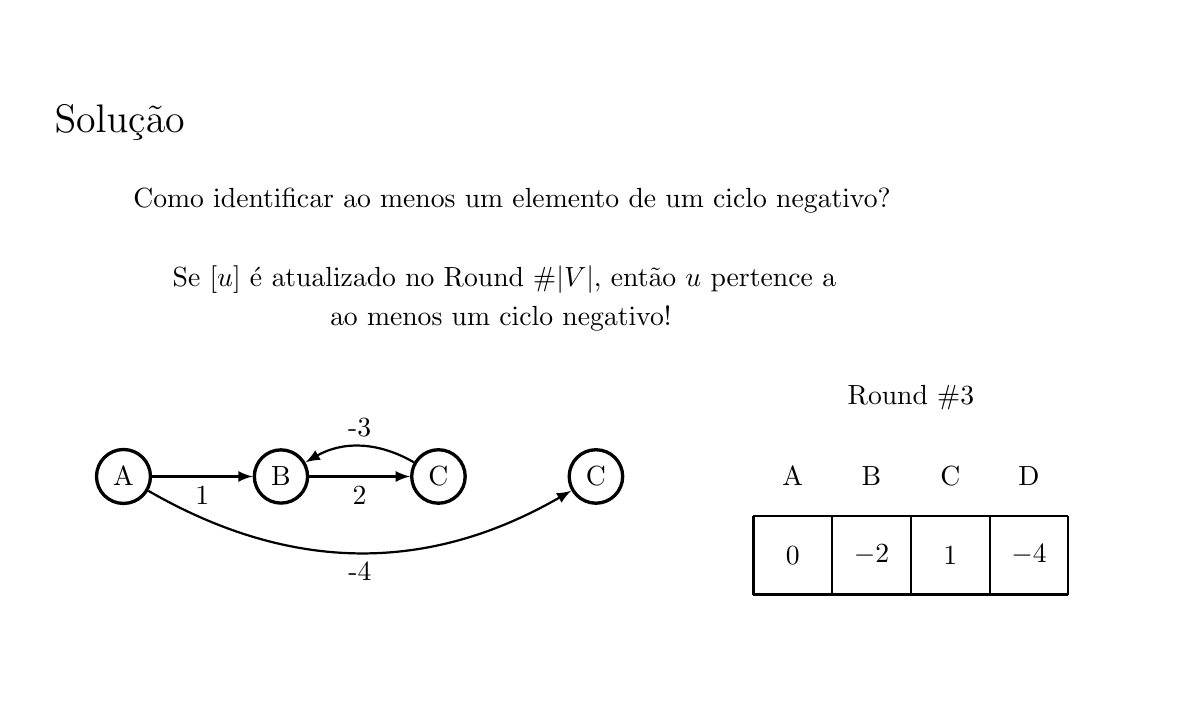
\begin{tikzpicture}
\node[draw,opacity=0] at (0, 0) {x};
\node[draw,opacity=0] at (14, 8) {x};
 \node[anchor=west] at (0, 7) { \Large \bbbold{Solução} };
 \node[anchor=west] at (1, 6) { \bbtext{Como identificar ao menos um elemento de um ciclo negativo? } };
 \node[anchor=west] at (1.5, 5) { \bbcomment{Se $\dist[u]$ é atualizado no Round \#$|V|$, então $u$ pertence a } };
 \node[anchor=west] at (3.5, 4.5) { \bbcomment{ao menos um ciclo negativo! } };
 \node[draw,very thick,circle] (A) at (1, 2.5) { \bbtext{A} };
 \node[draw,very thick,circle] (B) at (3, 2.5) { \bbtext{B} };
 \node[draw,very thick,circle] (C) at (5, 2.5) { \bbtext{C} };
 \node[draw,very thick,circle] (D) at (7, 2.5) { \bbtext{C} };
 \draw[-latex,thick] (A) to node[below] { \bbinfo{1} } (B);
 \draw[-latex,thick] (B) to node[below] { \bbinfo{2} } (C);
 \draw[-latex,thick] (C) to [bend right] node[above] { \bbinfo{-3} } (B);
 \draw[-latex,thick] (A) to [bend right] node[below] { \bbinfo{-4} } (D);
 \draw[thick] (9, 1) grid (13, 2);
 \node at (9.5, 2.5) { \bbtext{A} };
 \node at (10.5, 2.5) { \bbtext{B} };
 \node at (11.5, 2.5) { \bbtext{C} };
 \node at (12.5, 2.5) { \bbtext{D} };
 \node at (9.5, 1.5) { $0$ };
 \node at (12.5, 1.5) { $-4$ };
 \node at (11, 3.5) { \bbbold{Round \#3} };
 \node at (10.5, 1.5) { $-2$ };
 \node at (11.5, 1.5) { $1$ };
\end{tikzpicture}
\end{frame}

\begin{frame}[plain,t]
\begin{tikzpicture}
\node[draw,opacity=0] at (0, 0) {x};
\node[draw,opacity=0] at (14, 8) {x};
 \node[anchor=west] at (0, 7) { \Large \bbbold{Solução} };
 \node[anchor=west] at (1, 6) { \bbtext{Como identificar ao menos um elemento de um ciclo negativo? } };
 \node[anchor=west] at (1.5, 5) { \bbcomment{Se $\dist[u]$ é atualizado no Round \#$|V|$, então $u$ pertence a } };
 \node[anchor=west] at (3.5, 4.5) { \bbcomment{ao menos um ciclo negativo! } };
 \node[draw,very thick,circle] (A) at (1, 2.5) { \bbtext{A} };
 \node[draw,very thick,circle] (D) at (7, 2.5) { \bbtext{C} };
 \draw[-latex,thick] (A) to node[below] { \bbinfo{1} } (B);
 \draw[-latex,thick] (B) to node[below] { \bbinfo{2} } (C);
 \draw[-latex,thick] (C) to [bend right] node[above] { \bbinfo{-3} } (B);
 \draw[-latex,thick] (A) to [bend right] node[below] { \bbinfo{-4} } (D);
 \draw[thick] (9, 1) grid (13, 2);
 \node at (9.5, 2.5) { \bbtext{A} };
 \node at (10.5, 2.5) { \bbtext{B} };
 \node at (11.5, 2.5) { \bbtext{C} };
 \node at (12.5, 2.5) { \bbtext{D} };
 \node at (9.5, 1.5) { $0$ };
 \node at (12.5, 1.5) { $-4$ };
 \node at (11, 3.5) { \bbbold{Round \#4} };
 \node at (10.5, 1.5) { $\mathbf{-3}$ };
 \node at (11.5, 1.5) { $\mathbf{0}$ };
 \node[draw,very thick,circle,fill=BBCyan] (B) at (3, 2.5) { \bbtext{B} };
 \node[draw,very thick,circle,fill=BBCyan] (C) at (5, 2.5) { \bbtext{C} };
\end{tikzpicture}
\end{frame}

\begin{frame}[plain,t]
\begin{tikzpicture}
\node[draw,opacity=0] at (0, 0) {x};
\node[draw,opacity=0] at (14, 8) {x};
 \node[anchor=west] at (0, 7) { \Large \bbbold{Solução} };
\end{tikzpicture}
\end{frame}

\begin{frame}[plain,t]
\begin{tikzpicture}
\node[draw,opacity=0] at (0, 0) {x};
\node[draw,opacity=0] at (14, 8) {x};
 \node[anchor=west] at (0, 7) { \Large \bbbold{Solução} };
 \node[anchor=west] at (1, 6) { \bbtext{Em que casos a pontuação pode ser arbitrariamente grande?} };
\end{tikzpicture}
\end{frame}

\begin{frame}[plain,t]
\begin{tikzpicture}
\node[draw,opacity=0] at (0, 0) {x};
\node[draw,opacity=0] at (14, 8) {x};
 \node[anchor=west] at (0, 7) { \Large \bbbold{Solução} };
 \node[anchor=west] at (1, 6) { \bbtext{Em que casos a pontuação pode ser arbitrariamente grande?} };
 \node[anchor=west] at (1.5, 5) { \bbcomment{Quando há um caminho de um nó de um ciclo negativo até $N$! } };
\end{tikzpicture}
\end{frame}

\begin{frame}[plain,t]
\begin{tikzpicture}
\node[draw,opacity=0] at (0, 0) {x};
\node[draw,opacity=0] at (14, 8) {x};
 \node[anchor=west] at (0, 7) { \Large \bbbold{Solução} };
 \node[anchor=west] at (1, 6) { \bbtext{Em que casos a pontuação pode ser arbitrariamente grande?} };
 \node[anchor=west] at (1.5, 5) { \bbcomment{Quando há um caminho de um nó de um ciclo negativo até $N$! } };
 \node[anchor=west] at (1, 3) { \bbtext{E como posso identificar a existência ou não de tais caminhos? } };
\end{tikzpicture}
\end{frame}

\begin{frame}[plain,t]
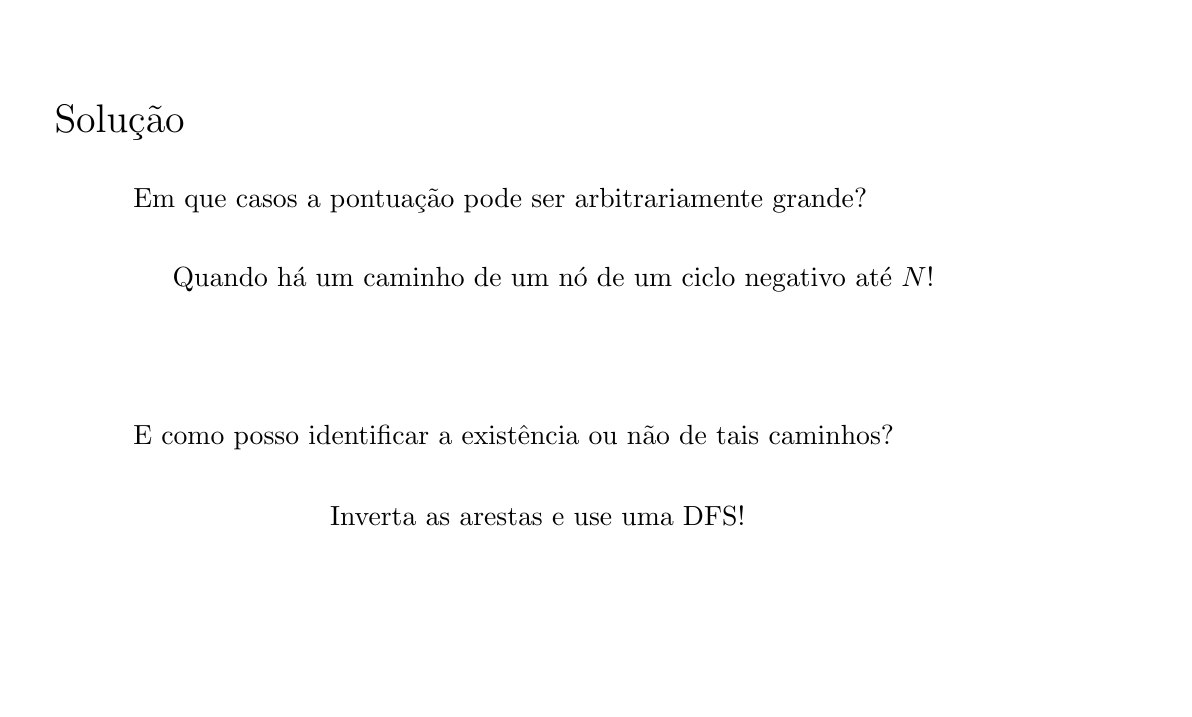
\begin{tikzpicture}
\node[draw,opacity=0] at (0, 0) {x};
\node[draw,opacity=0] at (14, 8) {x};
 \node[anchor=west] at (0, 7) { \Large \bbbold{Solução} };
 \node[anchor=west] at (1, 6) { \bbtext{Em que casos a pontuação pode ser arbitrariamente grande?} };
 \node[anchor=west] at (1.5, 5) { \bbcomment{Quando há um caminho de um nó de um ciclo negativo até $N$! } };
 \node[anchor=west] at (1, 3) { \bbtext{E como posso identificar a existência ou não de tais caminhos? } };
 \node[anchor=west] at (3.5, 2) { \bbcomment{Inverta as arestas e use uma DFS! } };
\end{tikzpicture}
\end{frame}

\begin{frame}[plain,t]
\begin{tikzpicture}
\node[draw,opacity=0] at (0, 0) {x};
\node[draw,opacity=0] at (14, 8) {x};
 \node[draw,very thick,circle] (A) at (3, 7) { \bbtext{A} };
 \node[draw,very thick,circle,fill=BBCyan] (B) at (5, 5) { \bbtext{B} };
 \node[draw,very thick,circle,fill=BBCyan] (C) at (5, 3) { \bbtext{C} };
 \node[draw,very thick,circle] (D) at (1, 5) { \bbtext{D} };
 \draw[-latex,thick] (A) to node[above right] { \bbinfo{3} } (B);
 \draw[-latex,thick] (A) to node[above left] { \bbinfo{2} } (D);
 \draw[-latex,thick] (B) to [bend left] node[right] { \bbinfo{3} } (C);
 \draw[latex-,thick] (B) to [bend right] node[left] { \bbinfo{-5} } (C);
\end{tikzpicture}
\end{frame}

\begin{frame}[plain,t]
 \inputsnippet{cpp}{9}{27}{codes/1112.cpp}
\end{frame}

\begin{frame}[plain,t]
 \inputsnippet{cpp}{29}{48}{codes/1112.cpp}
\end{frame}

\end{document}
